%!TEX root = ../dokumentation.tex

\section{Installationsschritte}

Die Projekte für „Client“ und „Server“ liegen jeweils als Eclipse Projekt vor.\\

\textbf{Client - Entwicklungsumgebung}

\begin{enumerate}
	\item Für die Entwicklungsumgebung der „Client“ Anwendung muss zunächst Eclipse IDE for Java Developers\footnote{http://www.eclipse.org/downloads/moreinfo/java.php} installiert werden.
	\item Das aktuelle Software Development Kit\footnote{http://developer.android.com/sdk/index.html\#ExistingIDE (Menü aufklappen)} muss geladen und entpackt werden
	\item Anschließend muss das „Android Development Tools“ Plugin\footnote{http://developer.android.com/sdk/installing/installing-adt.html} für Eclipse heruntergeladen und installiert werden.
	\item Der im Plugin enthaltene SDK Manager muss dann so konfiguriert werden, dass er den Pfad zu dem bereits heruntergeladen SDK kennt.
	\item Nach der Konfigration müssen weitere Tools und Pakete geladen werden, siehe Abb. \ref{fg:android-sdk-manager}.
	\begin{figure}[H]
		\centering
		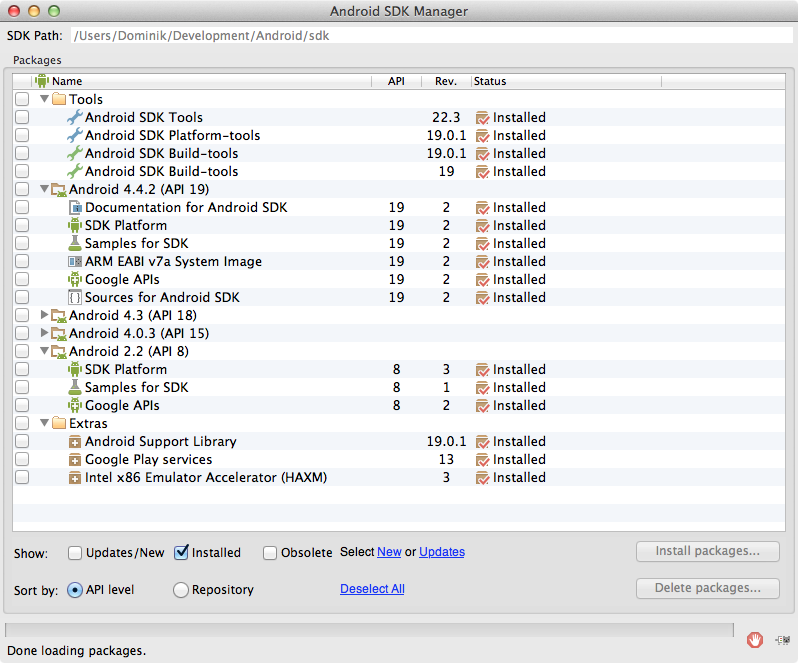
\includegraphics[width=0.85\textwidth]{./images/install/android-sdk-manager.png}
		\caption{SDK Manager: Pakete, die installiert werden müssen.}
		\label{fg:android-sdk-manager}
	\end{figure}
	\item Optional: Falls kein Testgerät vorliegt, welches den Anforderungen entspricht, kann ein „Android Virtual Device“ (AVD)\footnote{http://developer.android.com/tools/devices/index.html} eingerichtet werden. In unseren Tests hat sich ein AVD auf Basis des Nexus One (Abb. \ref{fg:android-adv}) als hilfreich erwiesen. Wichtig ist, dass bei \textit{Target} ein Wert mit \textit{Google APIs} als Präfix ausgewählt wird.
	\begin{figure}[H]
		\centering
		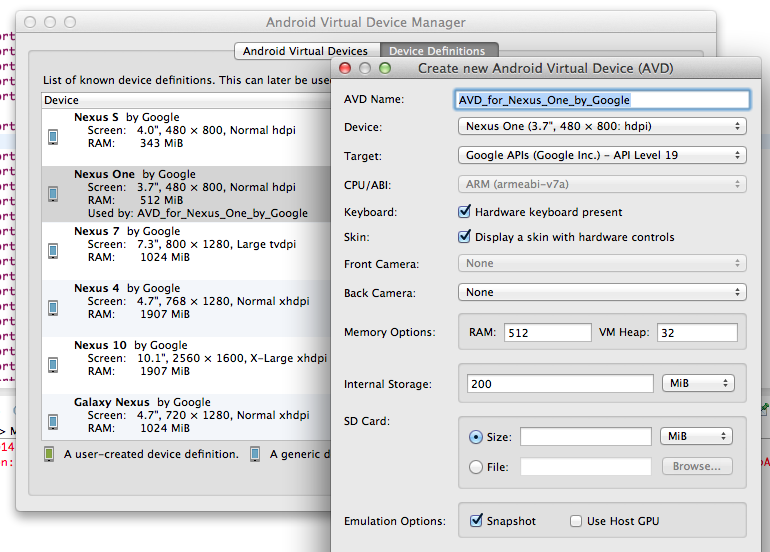
\includegraphics[width=0.85\textwidth]{./images/install/android-avd.png}
		\caption{AVD auf Basis des Nexus One}
		\label{fg:android-adv}
	\end{figure}
\end{enumerate}
